\documentclass[twocolumn,12pt]{article}
\usepackage[utf8]{inputenc}
\usepackage{lmodern} %fuente a utilizar
\usepackage{setspace}
\usepackage{geometry}
\usepackage{fancyhdr}
\usepackage{graphicx} % Paquete para manejar imágenes
\usepackage[absolute,overlay]{textpos} % Para posicionar la imagen
\usepackage{datetime2} % Para personalizar el formato de la fecha
\usepackage{amsmath}
\usepackage{amssymb}
\usepackage{graphicx}
\usepackage{multicol}
\geometry{
    a4paper,
    left=18mm,
    right=18mm,
    top=40mm, % Ajusta el margen superior si es necesario
    bottom=20mm,
    headsep=35mm, % Ajusta el espacio entre encabezado y texto
}


% Configuración de espaciado entre líneas
\setstretch{1.5}

% Define the header
\pagestyle{fancy}
\fancyhf{} % Clear all header and footer fields
\fancyhead[L]{
\vspace{-0.5cm}

\includegraphics[width=5cm]{Multimedia/logo_uai.png}} % Adjust the width as needed
\renewcommand{\headrulewidth}{0.5pt} % Line thickness for the header separator
\fancyfoot[C]{\thepage}

\begin{document}
	
	\begin{titlepage}
		\centering
                % Adjust vertical space to move the content higher
            \vspace*{-0.5in} % Reduced to move everything up
		\vspace*{1in}
		
		% Configuración de la imagen en la esquina superior derecha
		\begin{textblock*}{0in}(12.5cm,2cm) % (ancho del bloque, coordenada-x, coordenada-y)
			
\includegraphics[width=3in,height=3in,keepaspectratio]{./Multimedia/logo_uai.png}
		\end{textblock*}
		
		% Línea horizontal sobre el título
		\noindent\rule{1\textwidth}{0.4pt}
		\begin{flushleft}
			\textbf{FIS101}
		\end{flushleft}
		
		\vspace{0in} % Espacio entre la línea y el título
		
		% Título del Informe
		\begin{flushleft}
			\huge
			\textbf{Laboratorio 1\\}
			\large
			\textbf{Medición de la aceleración en caída libre:\\ aplicando el principio de Galileo}
			\vspace{0.4in} % Espacio entre el título y la línea inferior
		\end{flushleft}
		
		% Línea horizontal debajo del título
		\noindent\rule{1\textwidth}{0.4pt}
		
		\vspace{0.8in}
		
		% Información del informe
		\large
		\begin{flushleft}
			\textbf{Integrantes:}
			
			\begin{itemize}
				\item Ferré Díaz Felipe
				\item Muñoz Escobedo Benjamin 
                \item Quezada Escobar Víctor
			\end{itemize}
			
			\vspace{0.2in}
			
			\large
			\textbf{Curso:} Física I; Sección 1
			
			\vspace{0.2in}
			
			\large
			\textbf{Profesor:} David Aguayo Vera
		\end{flushleft}
		
		\vspace{0.2in}
		
		\begin{flushright}
			\Large
			Fecha: \today % Fecha actual en formato de año
		\end{flushright}
		
		
		
		\vspace{1in}
	\end{titlepage}
	
	% Secciones del documento
	\section{Resumen}
	Se debe escribir una vez tengamos los datos e informe completo
	
	\section{Introducción}
	En este laboratorio replicamos parte de los ejercicios experimentales realizados por Galileo Galilei en su investigación sobre la aceleración constante debido a la gravedad, con la diferencia de que contamos con el material tecnológico que fue facilitado por la Universidad. Galileo hipotetizó que un objeto en caída libre adquiría cantidades iguales de velocidad en tiempos iguales. Para lo anterior Galileo diseñó un experimento que consistía en una rampa donde deslizaría distintos pesos en distintos grados para comprobar que la taza de aceleración no dependía de las masas utilizadas. Contrastaremos los datos obtenidos experimentalmente con el marco teórico obtenido en las cátedras de Física I, principalmente con las ecuaciones itinerarios en los ejes "X" e "Y" referenciales, y el cálculo de su componente resultante según la suma trigonométrica de los vectores obtenidos.
		
	\section{Ecuaciones}
 	A continuación presentamos las ecuaciones bases utilizadas para los cálculos realizados en el marco teórico del experimento propuesto. De las ecuaciones itinerario en los ejes referenciales X e Y obtendremos las ecuaciones de aceleración y velocidad. En conjunto con las ecuaciones de transformación de coordenadas cartesianas a polares, obtendremos los valores teóricos de aceleración en distintos ángulos de lanzamiento de nuestro carro a través de la rampa.
 	\vspace{-0.5cm}
 	\begin{center}

 	\begin{equation}
 		\centering
 		x_{(t)} = y_{0} + V_{0} \cdot t + a \cdot t^{2} 
 		\tag*{(1)} % ecuación itinerario eje x
 	\end{equation}
 		
 	\vspace{-0.5cm}
 	
 	\begin{equation}
 		\centering
 		y_{(t)} = y_{0} + V_{0} \cdot t + a \cdot t^{2} \tag*{(2)} % ecuación itinerario eje y
 	\end{equation}
 	
 	\vspace{-0.4cm}  
 	
	\centering\text{Ec. itinerarios relativa a los ejes x e y.}
	
	\begin{equation}
		\centering
		x = r \cdot Cos (\Theta) \tag*{(3)} 
	\end{equation}
	
	\vspace{-0.4cm}
	
	\begin{equation}
		\centering
		y = r \cdot Sen (\Theta) \tag*{(4)} 
	\end{equation}
	
	\vspace{-0.4cm}  
	
	\centering\text{Ec. conversión de coordenadas}
	\centering\text{polares a cartesianas.}
	
	\begin{equation}
	\centering
	r = \sqrt{x^{2} + y^{2}} \tag*{(5)} 
	\end{equation}
	\vspace{-0.4cm}
	\begin{equation}
	\centering
	\Theta = tan^{-1} \cdot \left( \frac{y}{x} \right) \tag*{(6)} 
	\end{equation}
	\vspace{-0.4cm}  
	\centering\text{Ec. conversión de coordenadas}
	\centering\text{cartesianas a polares.}
	\end{center}
	
	\vspace{1cm}
	
	De las ecuaciones anteriores podemos obtener, considerando el riel como referencia para nuestro eje x, y el eje y perpendicular al riel, las siguientes ecuaciones que nos permitirán calcular las aceleraciones, velocidades y ecuaciones itinerario resultantes y compararlos con los datos obtenidos en el ejercicio experiemental.
	\vspace{-1cm}
	\begin{center}
	\begin{equation}
	\centering
	a_{x} = g \cdot Sen (\Theta) \tag*{(7)} 
	\end{equation}
	
	\vspace{-0.4cm}  
	
	\centering\text{Ec. aceleración en el eje x.}
	\end{center}
	
	Debido a que estamos en un plano inclinado, tomado como ejes referenciales, se presenta la ecuación 7, con a como aceleracion en el eje x, g, gravedad mediad por los intrumentos de laboratorio y $\Theta$ el ángulo del riel con respecto a la mesa horizontal donde está ubicada.
	\vspace{-0.5cm}
	\begin{center}
	\begin{equation}
	\centering
	v_{x(t)} = v_{0} + a_{x}\cdot t \tag*{(9)} 
	\end{equation}
	
	\vspace{-0.4cm}  
	
	\centering\text{Ec. velocidad vs tiempo a lo largo del eje x.}
	
		\begin{equation}
	\centering
	x_{(t)} = x_{0} + v_{0} \cdot t + \left( \frac{1}{2} \right) \cdot a_{x}\cdot t^{2} \tag*{(10)} 
	\end{equation}
	
	\vspace{-0.4cm}  
	
	\centering\text{Ec. posicion vs tiempo a lo largo del eje x.}
	\end{center}

        Deducimos de las a fórmulas itinerario la formula para calcular la velocidad final tomando datos teóricos y practicos descritos a continuación:
	
	\[
	v_f = \sqrt{v_i^2 + 2 \cdot a \cdot x}
	\]
	
	Donde:
	\begin{itemize}
		\item \(v_f\) es la velocidad final en el punto B (en metros por segundo, m/s).
		\item \(v_i\) es la velocidad inicial en el punto A (valor práctico obtenido del las grabaciones, en metros por segundo, m/s).
		\item \(a\) es la aceleración a lo largo del plano inclinado (valor calculado en base a las lecturas del acelerómetro y el cálculo de las componentes de x e y de la gravedad en metros por segundo al cuadrado, m/s²).
		\item \(x\) es el desplazamiento a lo largo del plano inclinado desde el punto A hasta el punto B (en metros, m).
	\end{itemize}
	
	\section{Metodología}
	El experimento consistió en posicionar un carro y dezlizarlo sobre un plano inclinado. Utilizamos la cámara de nuestros celulares para grabar la caída y procesar el video en el software propuesto por el profesor y obtener los graficos de posición y velocidad para diferentes angulos del riel en referencia sobre el plano horizontal. Los materiales utilizados para el experimento fueron los siguientes:
	
	\begin{enumerate}
	\item Riel Pasco.
	\item Carro de colisiones Pasco.
	\item Indicador de ángulo Pasco.
	\item Masa adicional.
	\item Balanza digital.
	\item Acelerómetro PocketLab.
	\item Teléfono celular para grabar video.
	\item Computador con el software Tracker. 
	\item Regla metálica.
	\end{enumerate}	
	
	\begin{figure}[h]
	\centering
	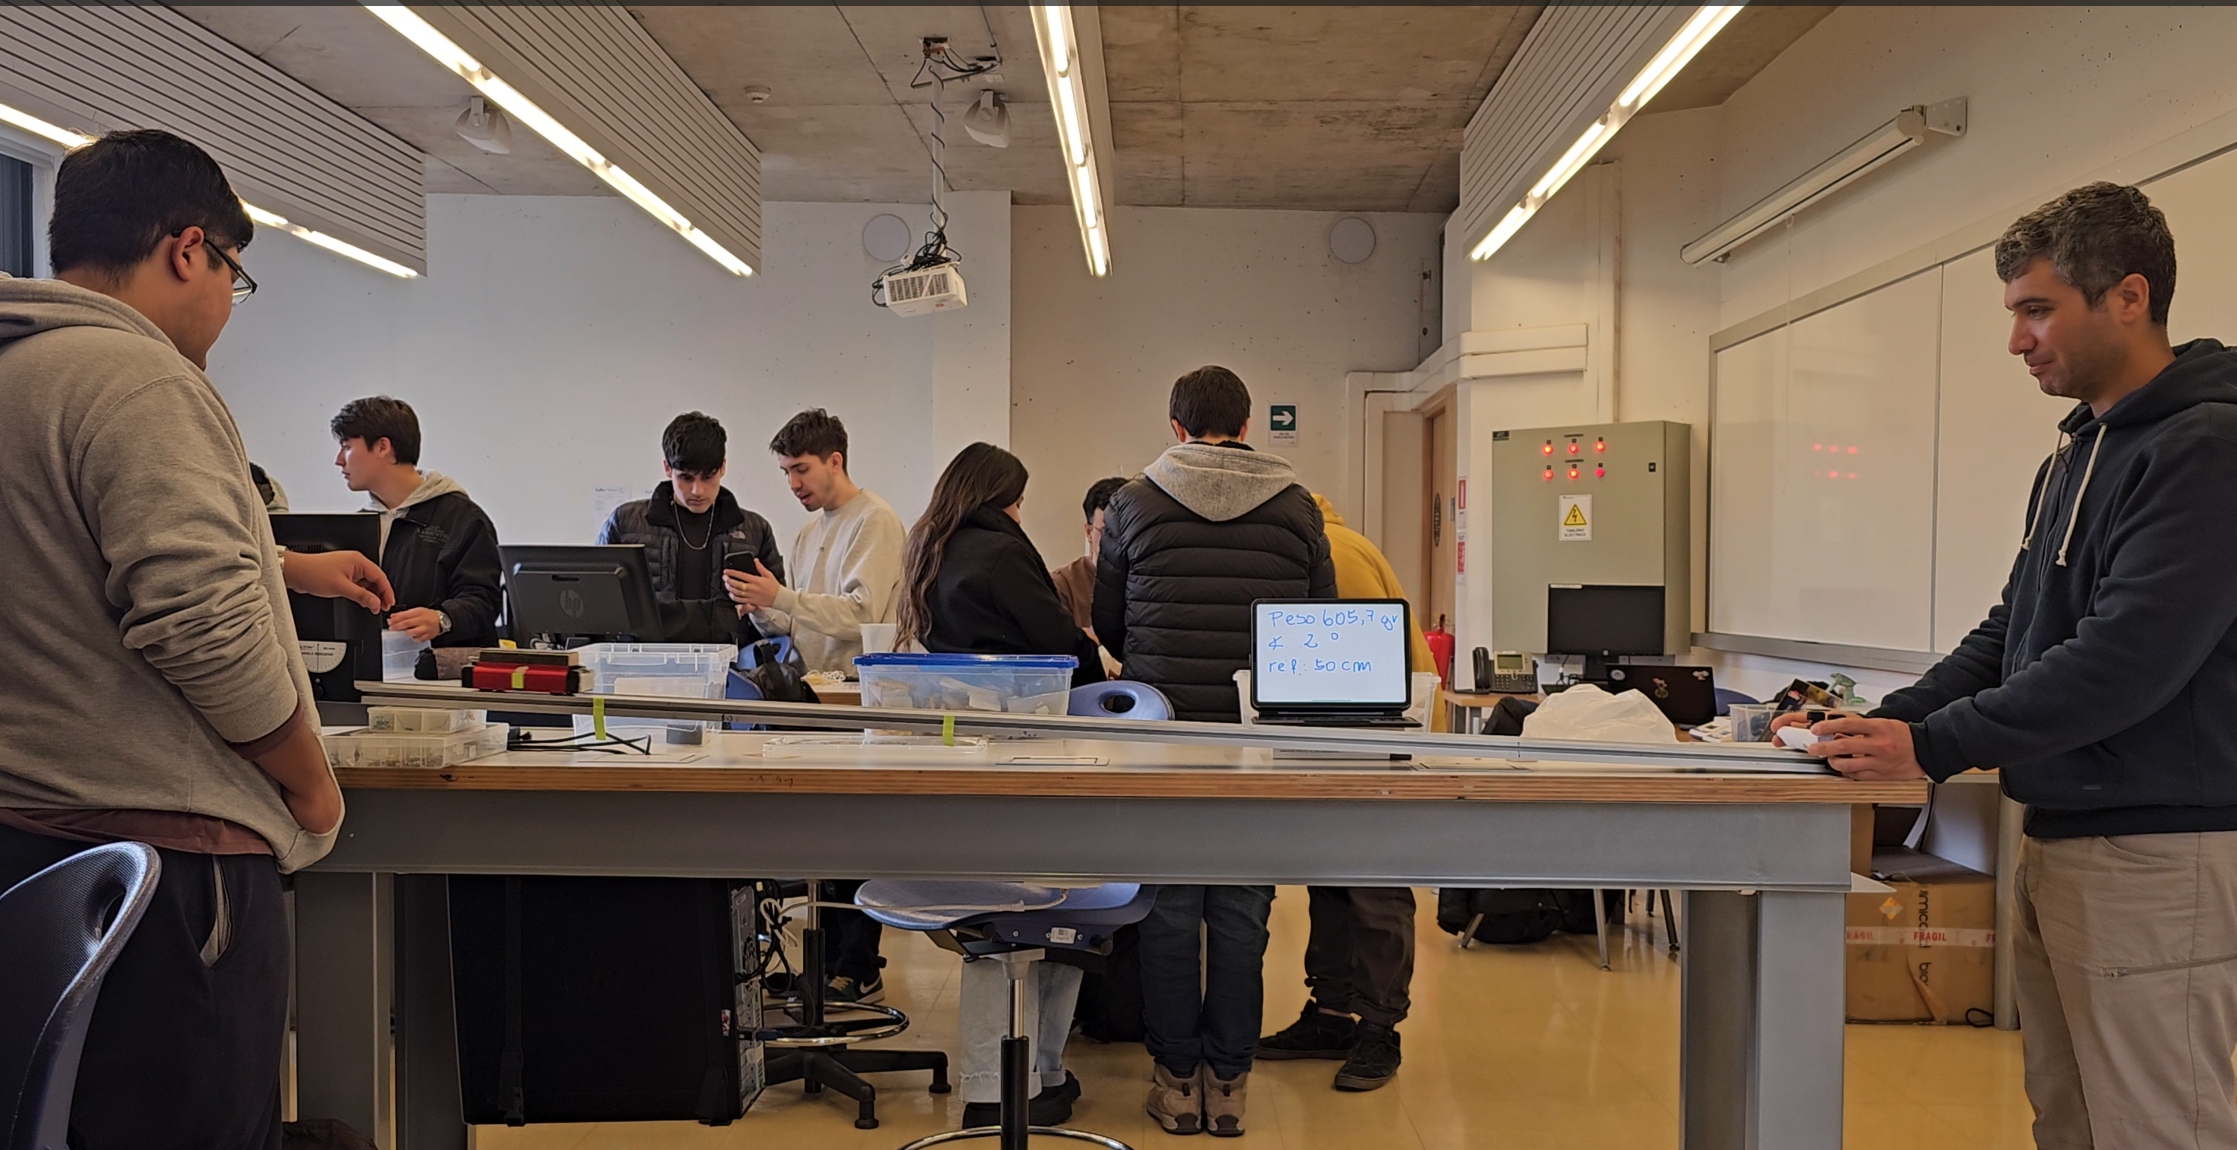
\includegraphics[width=0.5\textwidth]{./Multimedia/fotografia_laboratorio.png}
	\caption{ Procedimiento experimental}
	\label{Imagen:mi_imagen}
	\end{figure}
	
	\section{Resultados}
	blabla
	
	\subsection{Tablas}

	\onecolumn
	\begin{table}[h!]
	\centering
	\begin{tabular}{|c|c|c|}
	\hline
	\textbf{Ángulo de inclinación} & \multicolumn{2}{c|}{\textbf{Aceleración del cuerpo [m/s\(^2\)]}} \\ \cline{2-3}
	\textbf{} & \textbf{Sin masa adicional} & \textbf{Con masa adicional} \\ \hline
	2\textdegree & 0.371 & 0.373 \\ \hline
	4\textdegree & 0.695 & 0.697 \\ \hline
	8\textdegree & 1.24 & 1.26 \\ \hline
	10\textdegree & 1.68 & 1.69 \\ \hline
	14\textdegree & 2.37 & 2.37 \\ \hline
	\end{tabular}
	\caption{Tabla de aceleraciones experimentales en función del ángulo de inclinación.}
	\label{tabla:aceleraciones}
	\end{table}
	
	\begin{table}[h!]
	\centering
	\begin{tabular}{|c|c|c|}
	\hline
	\textbf{Ángulo de inclinación} & \textbf{Aceleración [m/s\(^2\)]} & \textbf{Velocidad final [m/s]} \\ \hline
	2\textdegree & 0.342 & 1.17 \\ \hline
	4\textdegree & 0.684 & 1.65 \\ \hline
	8\textdegree & 1.36 & 2.33 \\ \hline
	10\textdegree & 1.71 & 2.62 \\ \hline
	14\textdegree & 2.37 & 3.08 \\ \hline
	\end{tabular}
	\caption{Tabla de aceleraciones y velocidades teoricas en función del ángulo de inclinación.}
	\label{tabla:caida_galileo}
	\end{table}

        \begin{table}[h!]
		\centering

		\begin{tabular}{|c|c|c|c|c|c|c|}
			\hline
			\rowcolor{white} % Color de fondo para la primera fila
			Grados & Acel. Teo. en x & V_{A} Pract.  & V_{B} Pract. & V_{B} Teo. & V_{f} Teo-Pract. & V_{f} teo \\ \hline
			2 grados & 0,342 [m/s^{2}] & 0,555 [m/s] & 0,788 [m/s] & 0,624 [m/s] & Valor & Valor \\ \hline
			4 grados & 0,684 [m/s^{2}] & 0,747 [m/s] & 1,095 [m/s] & 3,773 [m/s]& Valor & Valor \\ \hline
			8 grados & 1,360 [m/s^{2}] & 1,004 [m/s] & 1,405 [m/s] & 5,311 [m/s]& Valor & Valor \\ \hline
			10 grados & 1,710 [m/s^{2}] & 1,126 [m/s] & 1,677 [m/s] & 5,955 [m/s] & Valor & Valor \\ \hline
			14 grados & 2,370 [m/s^{2}] & 1,349 [m/s] & 2,105 [m/s] & 7,016 [m/s] & Valor & Valor \\ \hline
		\end{tabular}
		\caption{Tabla de comparación de velocidades teóricas y prácticas en A, B y final.}
		\label{tabla:caida_galileo}
	\end{table}

    \onecolumn
    \section{Gráficos}
    
    % Cambiar a una sola columna
    
    \begin{figure}[h]
        \centering
        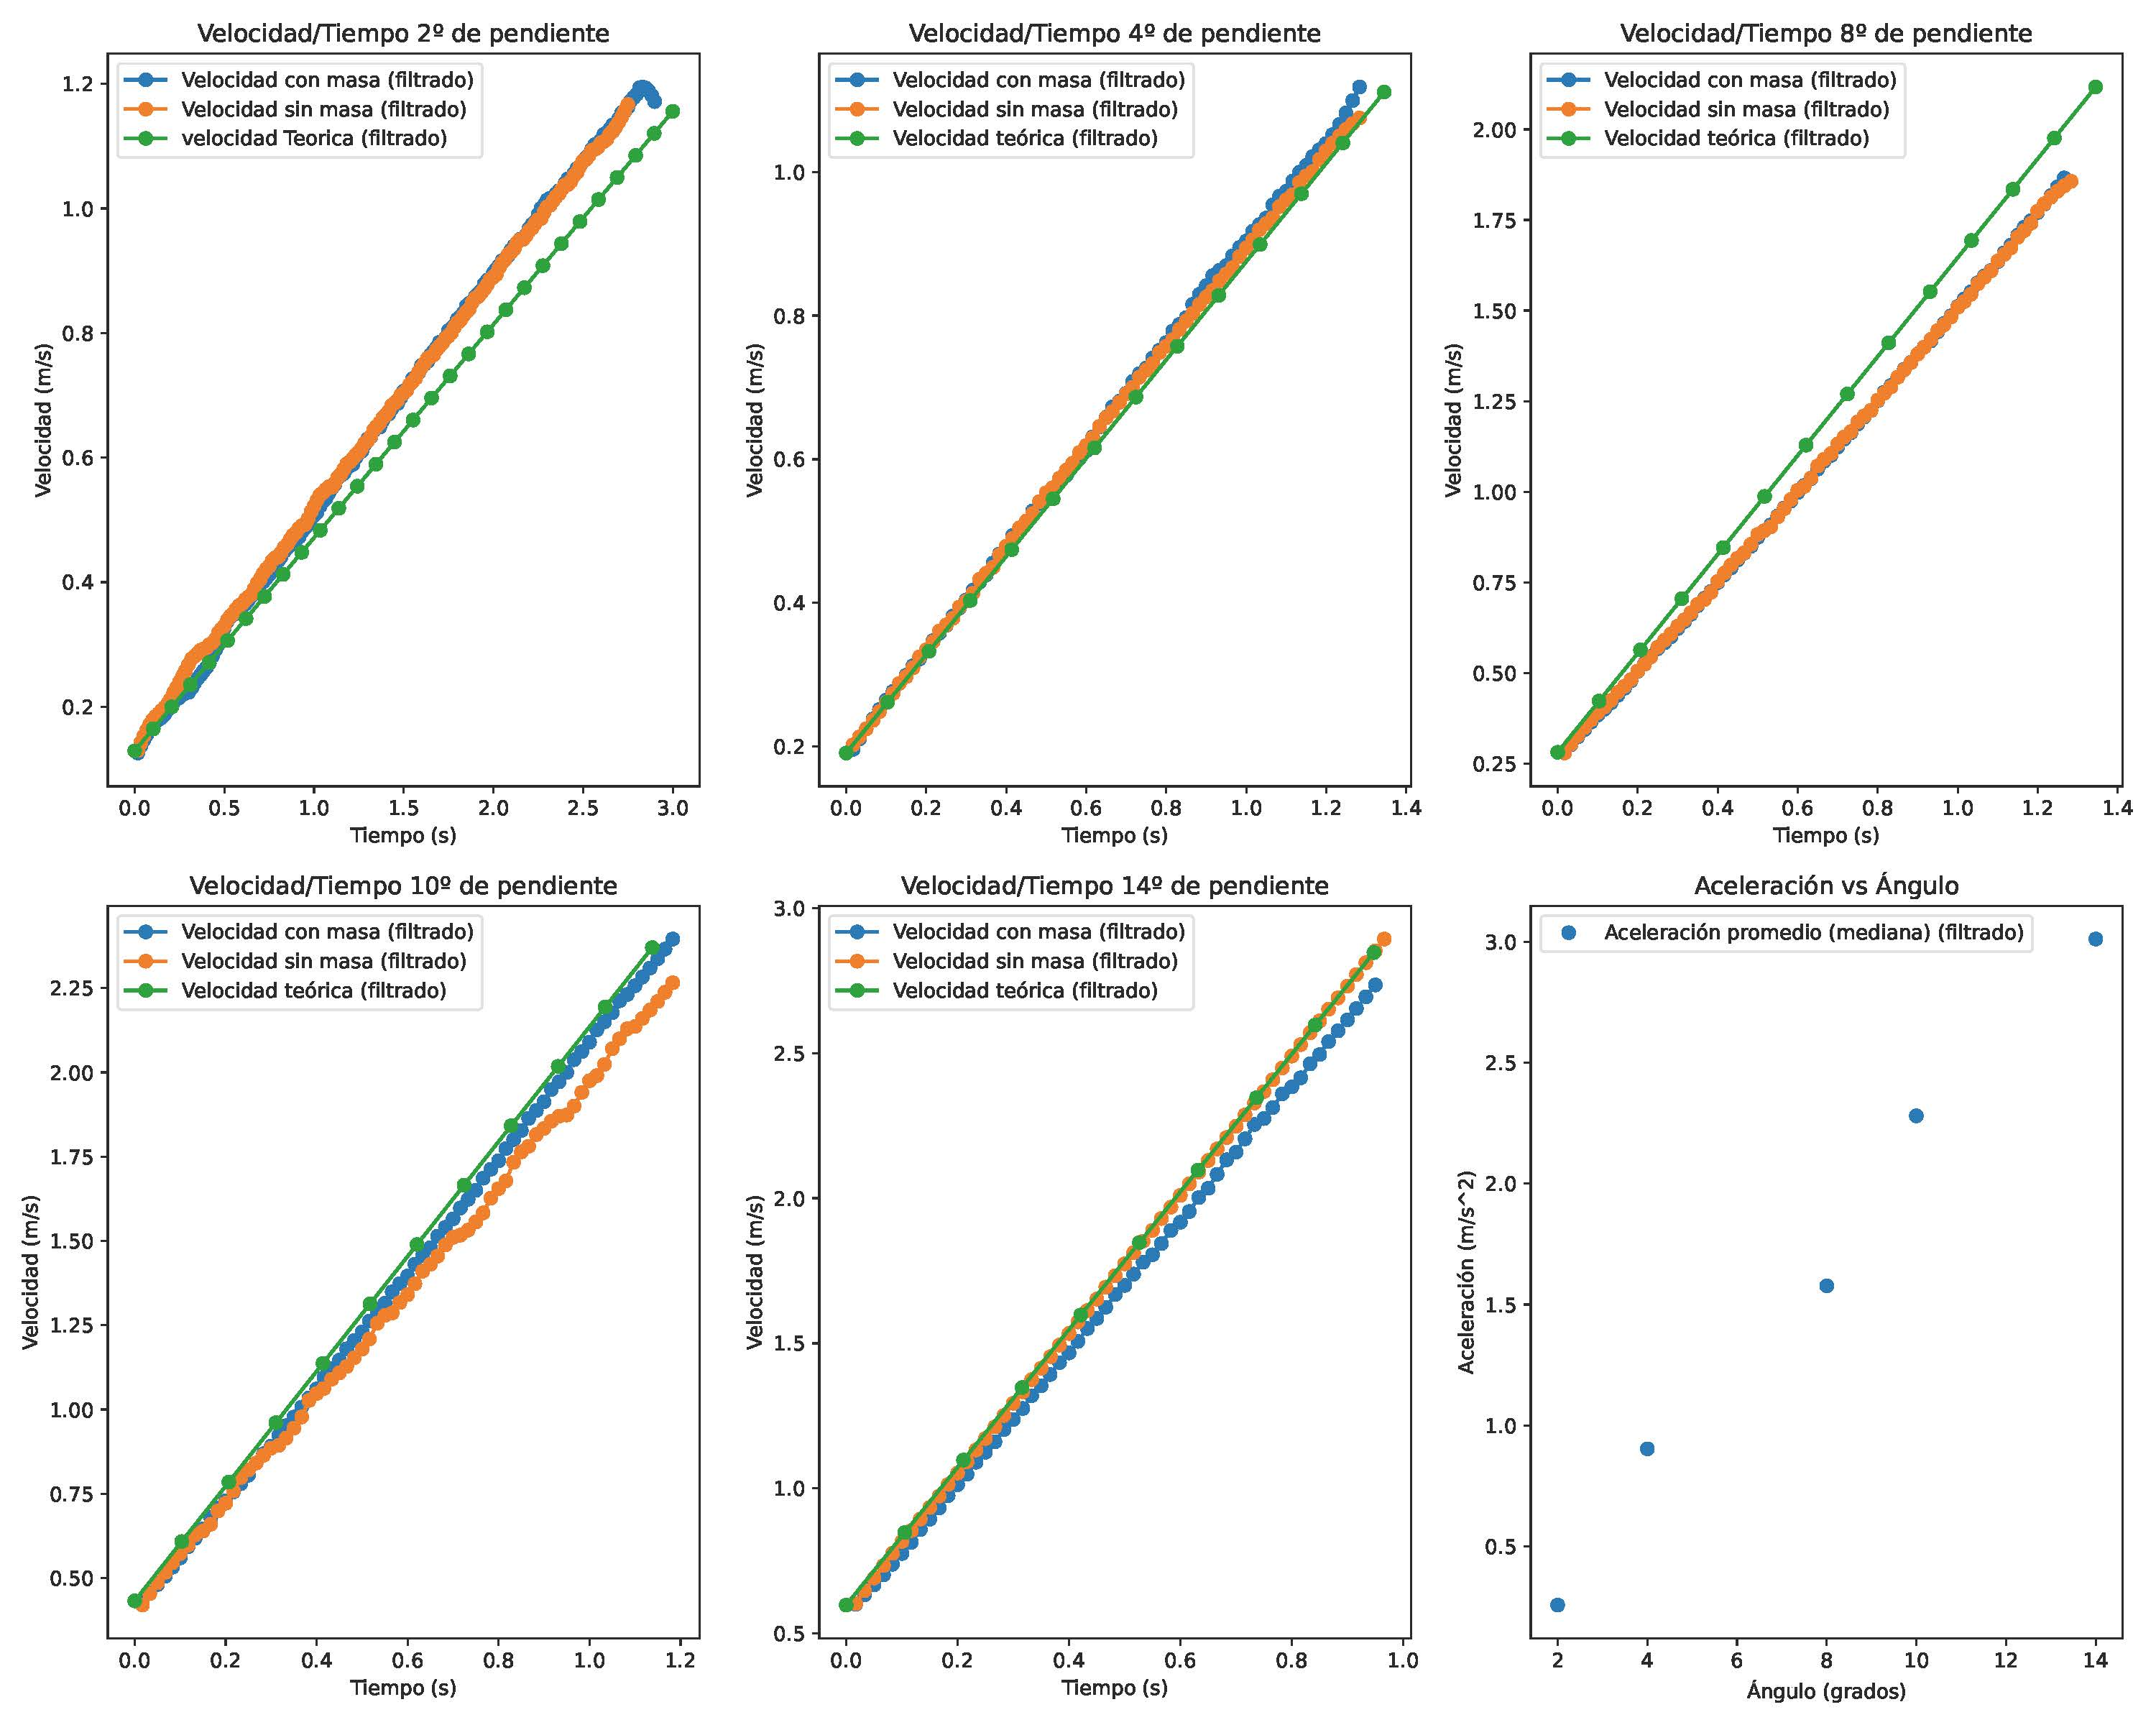
\includegraphics[width=0.8\textwidth]{Lab1/Multimedia/grafico1.jpg}
        \caption{Velocidad/Tiempo y aceleración/Ángulo.}
        \label{fig:imagen}
    \end{figure}

    \twocolumn
    
    \section{Discusión de resultados}
    blabla
    
    \subsection{Interpretación de los resultados}
    blabla.
    
    \subsection{Análisis de errores}
    blabla.
    
    \subsection{Comparación con la teoría}
    blabla.
    
    \subsection{Conclusiones}
    blabla.
    
    \section{Referencias bibliográficas}
    blabla.
    

	
	\section{Discusión de resultados}
	blabla
	
	\subsection{Interpretación de los resultados}
	blabla.
	
	\subsection{Análisis de errores}
	blabla.
	
	\subsection{Comparación con la teoría}
	blabla.
	
	\subsection{Conclusiones}
	blabla.
	
	
	\section{Referencias bibliográficas}
	Lista todas las fuentes consultadas y citadas en el informe. Utiliza un formato de citación apropiado según las normas académicas o el estilo requerido (por ejemplo, APA, MLA).

\end{document}

